\section{exercise h}

In this exercise we where going to simulate the nonlinear diffusion of Gaussian function

\begin{equation}
 I(x,y) = e^{-\frac{1}{2\sigma^2} \left( x^2 + y^2 \right)}
 \label{eq:gaussian}
\end{equation}

As we can see from figure \ref{fig:ex_h_start}, \ref{fig:ex_h_50_dt} and \ref{fig:ex_h_50_end}, the Gaussian is diffusing out into the plane and eventually all the grid points will
have the same value of $u(x,y)$.

\begin{figure}[h]
\begin{center}
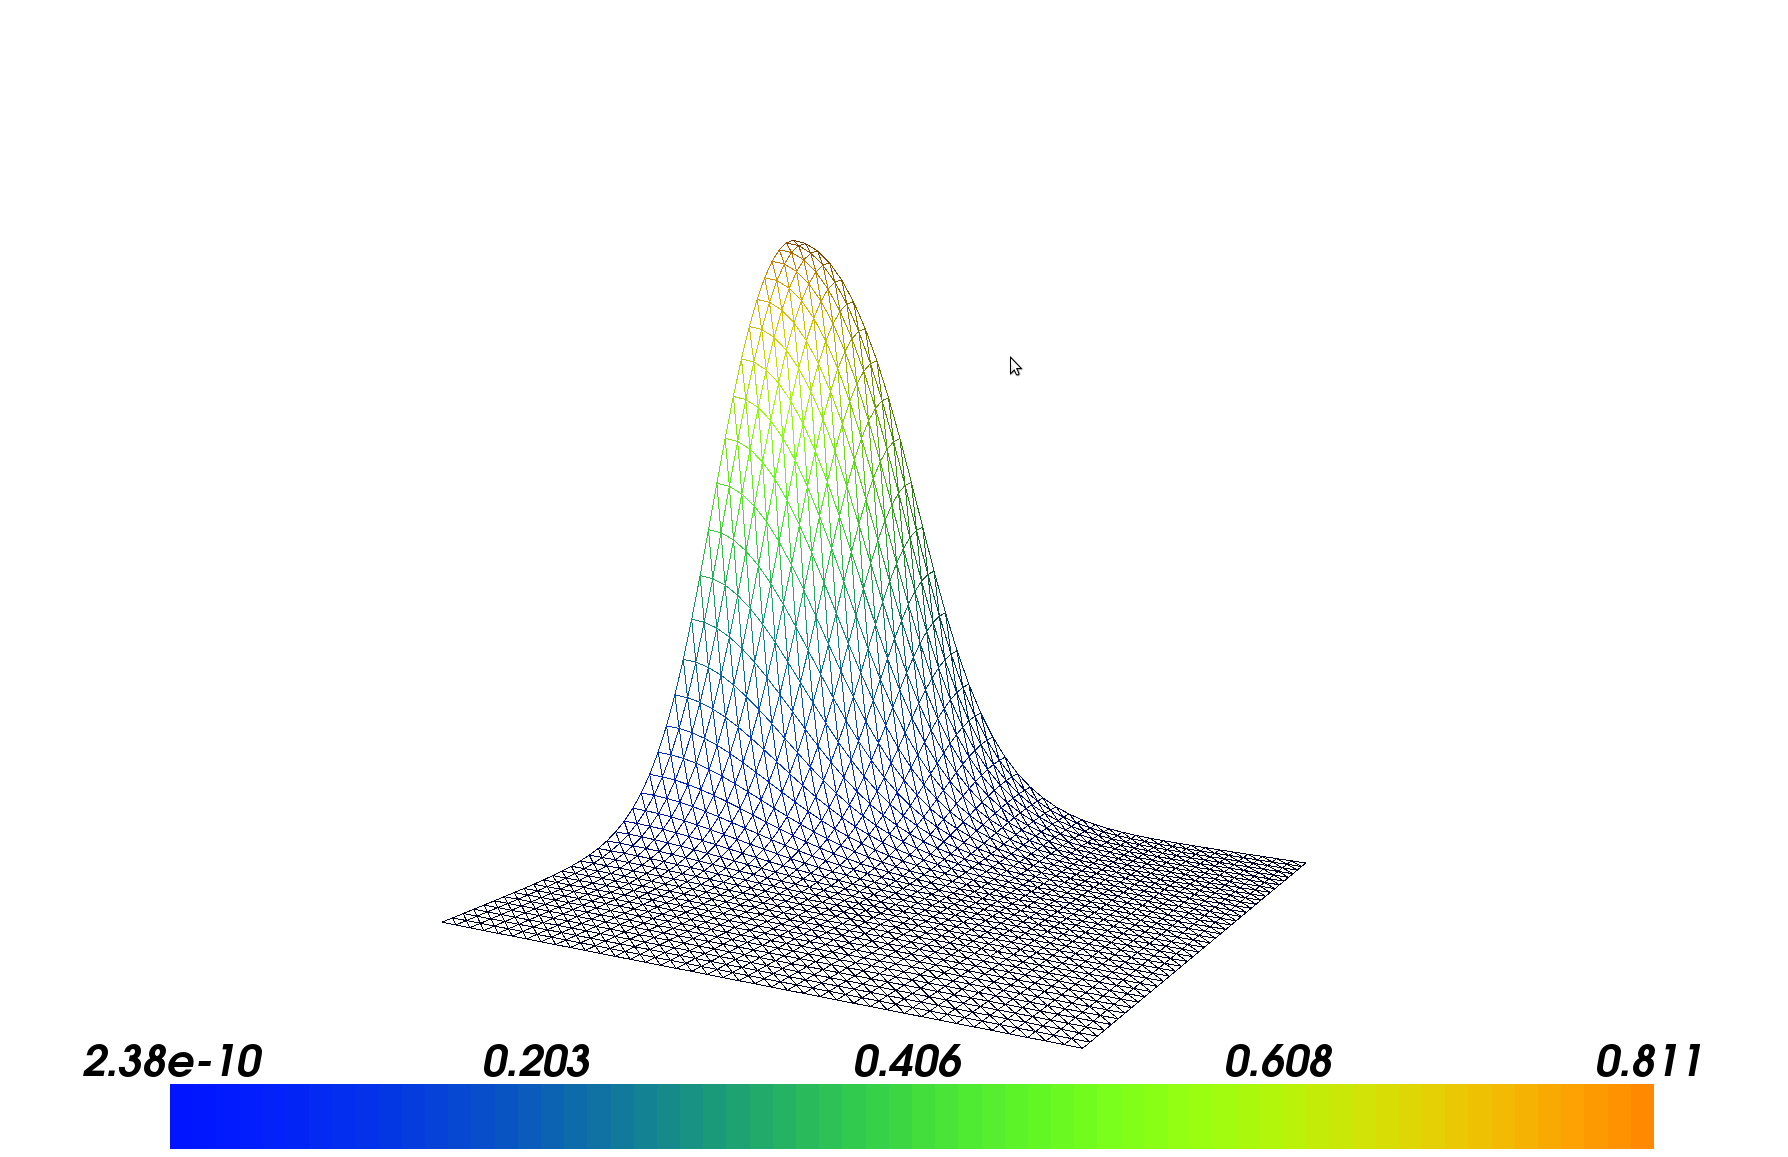
\includegraphics[scale=0.2]{images/ex_h_start.png}
\end{center}
\caption{The plot shows the the two dimensional Gaussian function \eqref{eq:gaussian} at the star of the simulation for $\sigma = 50$}
\label{fig:ex_h_start}
\end{figure}

\begin{figure}[h]
\begin{center}
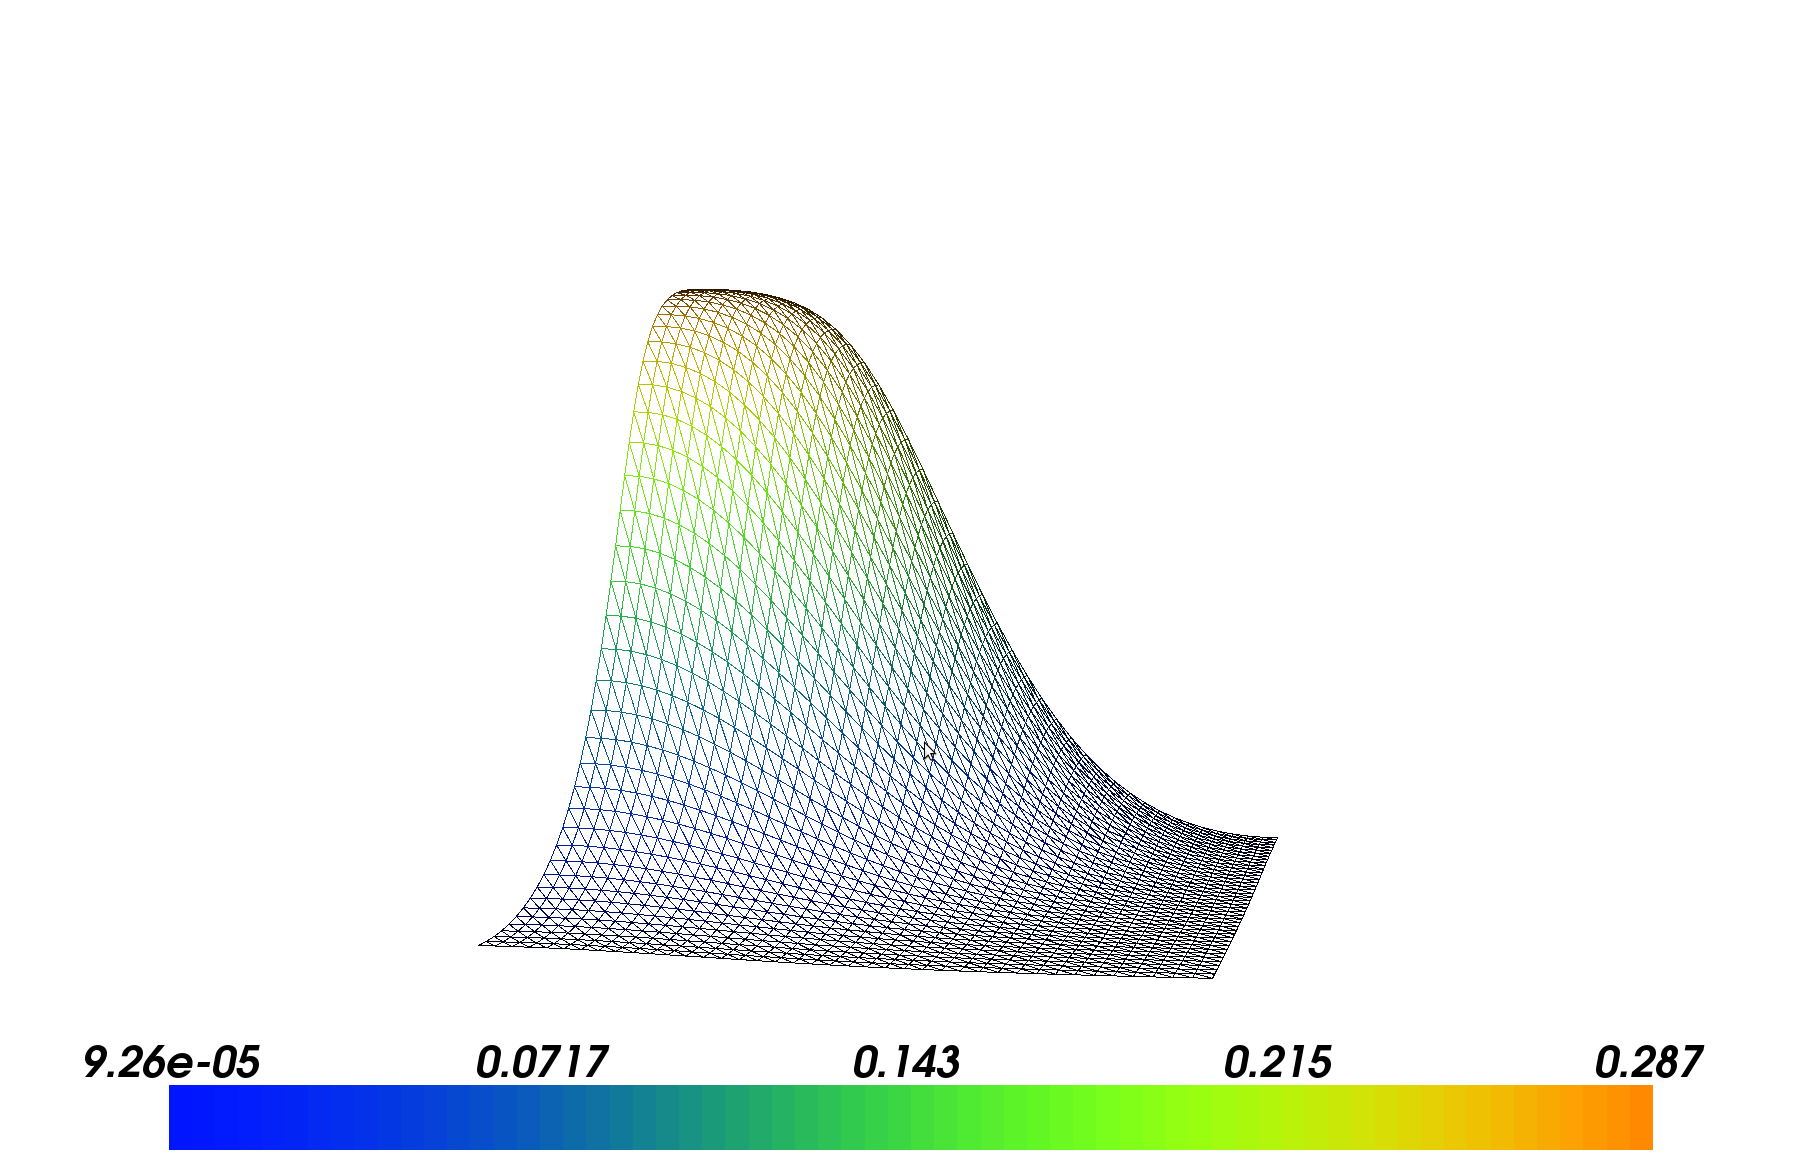
\includegraphics[scale=0.2]{images/ex_h_50_dt.png}
\end{center}
\caption{The plot shows the the two dimensional Gaussian function \eqref{eq:gaussian} after $50 dt$ for $\sigma = 50$}
\label{fig:ex_h_50_dt}
\end{figure}

\begin{figure}[h]
\begin{center}
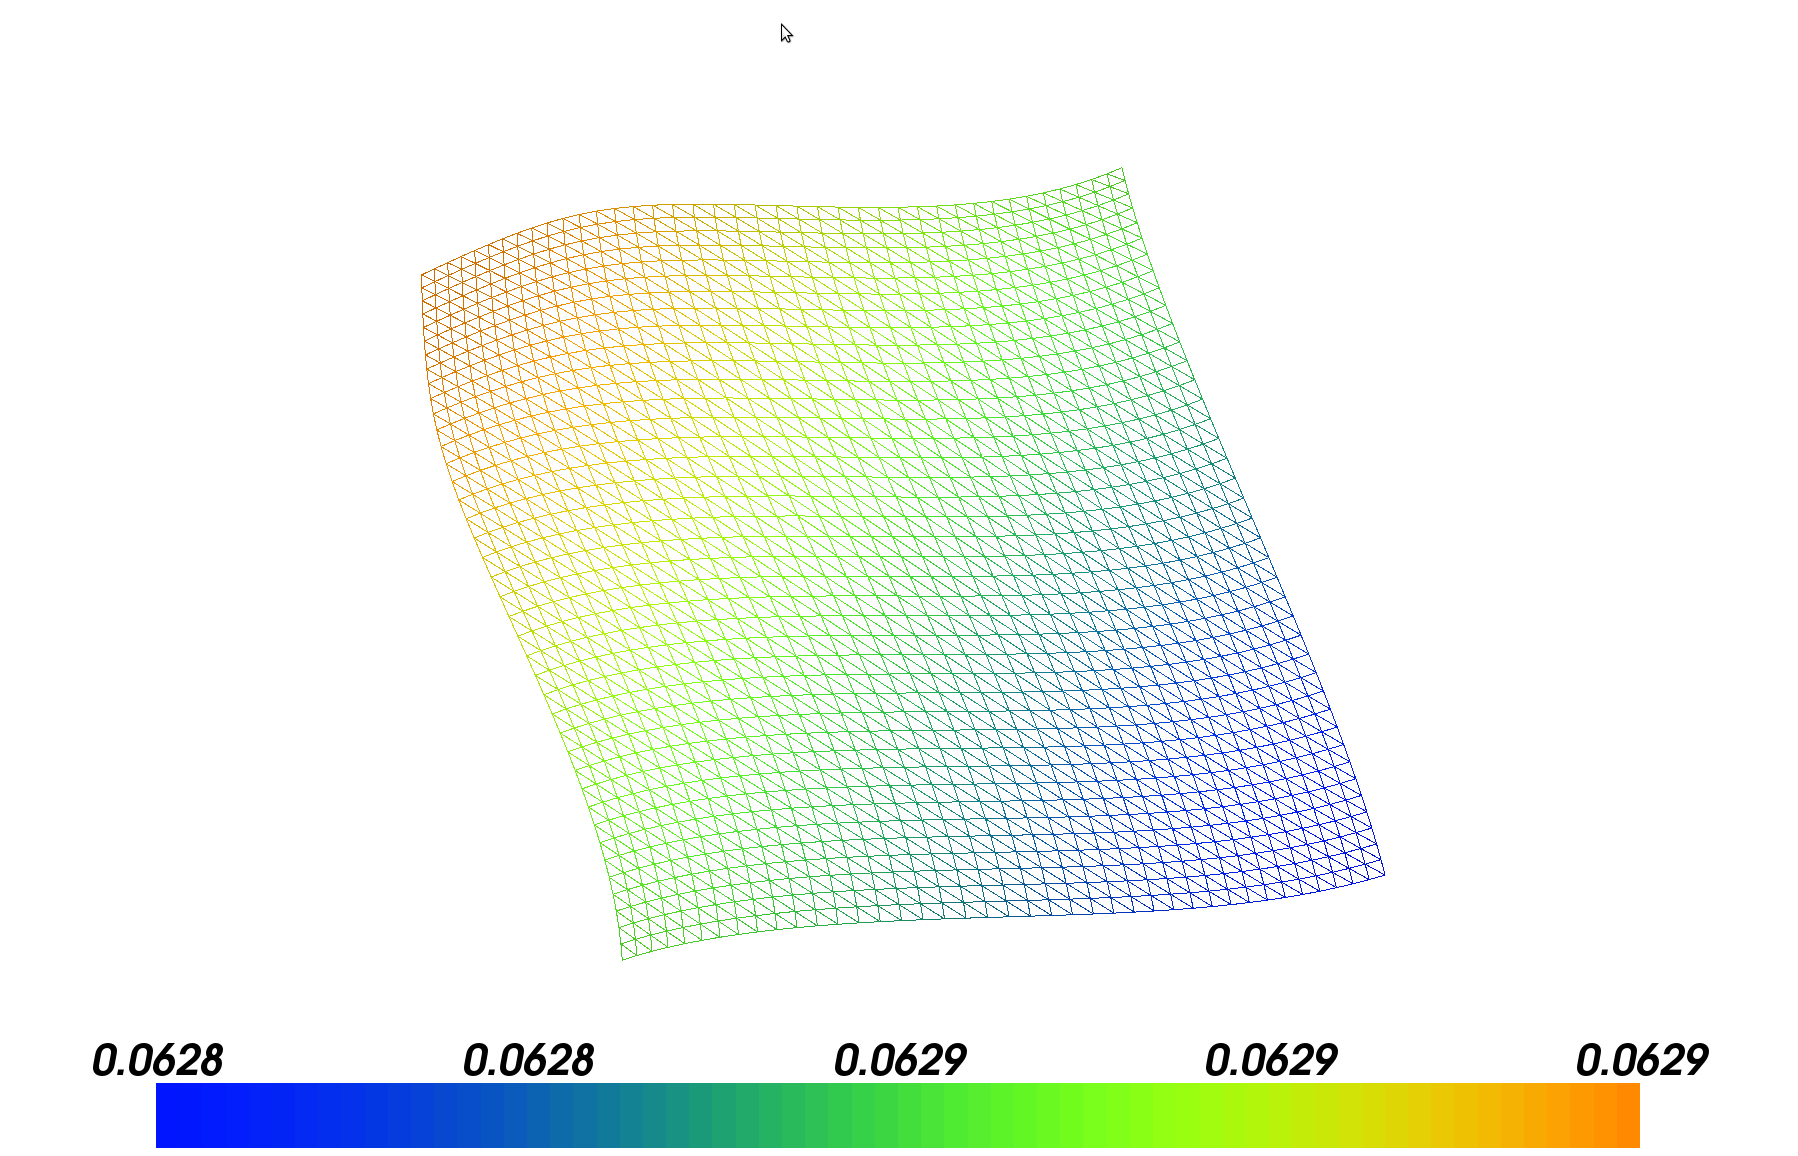
\includegraphics[scale=0.2]{images/ex_h_50_end.png}
\end{center}
\caption{The plot shows the the two dimensional Gaussian function \eqref{eq:gaussian} at the end of the simulation after $50 dt$ for $\sigma = 50$}
\label{fig:ex_h_50_end}
\end{figure}
